% Copyright © 2017 Christopher Helmes <helmes@hiskp.uni-bonn.de>
% Licensed under CC-BY 4.0

\documentclass{scrartcl}

\pagestyle{empty}

\usepackage{tikz}
\usepackage{amsmath,dsfont}

\usetikzlibrary{decorations}
\usetikzlibrary{decorations.markings}

\begin{document}


 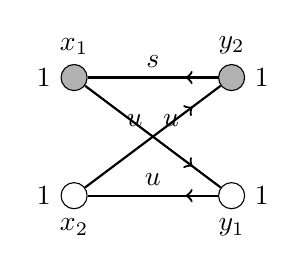
\begin{tikzpicture}[node distance=1.5cm]
 	% A picture showing the direct diagram of a 4pt correlation function. Need two vertices at tf and ti, and four quarklines, also the vertices should be named with the vertex factors and tf and ti as well 
 	% Vertices: Two Kaon vertices and two pion vertices. represent with filled, empty circle
 	% style for nodes
 	% styles for the mesons
 	\tikzstyle{strange}=[shape=circle, draw=black, fill=black!30]
 	\tikzstyle{light}=[shape=circle, draw=black]
 	% styles for the quarklines
 	\tikzstyle{itof}=[thick,decoration={markings,mark=at position 0.25 with {\arrow{>}}},postaction=decorate]
 	\tikzstyle{ftoi}=[thick,decoration={markings,mark=at position 0.25 with {\arrow{<}}},postaction=decorate]
 
 	\node[strange] at (0,0.5) (k_ti)[label=above:$x_1$,label=left:$\mathds{1}$] 		 			{};
 	\node[light] (pi_ti) 			[below of=k_ti,label=below:$x_2$,label=left:$\mathds{1}$] {};
 	\node[strange] at (2,0.5) (k_tf)[label=above:$y_2$,label=right:$\mathds{1}$] 		 			{}
 	
 	edge [itof] node[auto,swap]{$s$}(k_ti)
 	edge [ftoi] node[auto,swap]{$u$}(pi_ti);
 	\node[light] (pi_tf) 			[below of=k_tf,label=below:$y_1$,label=right:$\mathds{1}$] {}
 	edge [ftoi] node[auto,swap]{$u$}(k_ti)
 	edge [itof] node[auto,swap]{$u$}(pi_ti);
 	
 	% Quarkline 1
 	%\draw (0,0 .. (2,0);
 \end{tikzpicture}

\end{document}
